% Created by tikzDevice version 0.10.1.2 on 2018-04-18 11:35:08
% !TEX encoding = UTF-8 Unicode
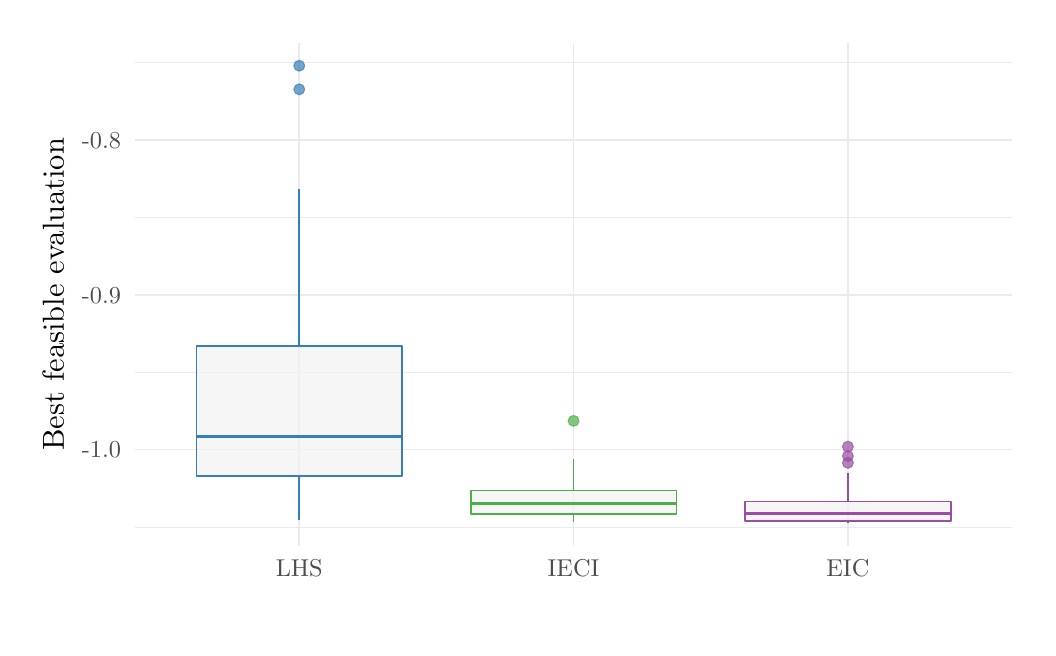
\begin{tikzpicture}[x=1pt,y=1pt]
\definecolor{fillColor}{RGB}{255,255,255}
\path[use as bounding box,fill=fillColor,fill opacity=0.00] (0,0) rectangle (361.35,216.81);
\begin{scope}
\path[clip] ( 38.67, 29.59) rectangle (355.85,211.31);
\definecolor{drawColor}{gray}{0.92}

\path[draw=drawColor,line width= 0.3pt,line join=round] ( 38.67, 36.38) --
	(355.85, 36.38);

\path[draw=drawColor,line width= 0.3pt,line join=round] ( 38.67, 92.32) --
	(355.85, 92.32);

\path[draw=drawColor,line width= 0.3pt,line join=round] ( 38.67,148.26) --
	(355.85,148.26);

\path[draw=drawColor,line width= 0.3pt,line join=round] ( 38.67,204.19) --
	(355.85,204.19);

\path[draw=drawColor,line width= 0.6pt,line join=round] ( 38.67, 64.35) --
	(355.85, 64.35);

\path[draw=drawColor,line width= 0.6pt,line join=round] ( 38.67,120.29) --
	(355.85,120.29);

\path[draw=drawColor,line width= 0.6pt,line join=round] ( 38.67,176.23) --
	(355.85,176.23);

\path[draw=drawColor,line width= 0.6pt,line join=round] ( 98.14, 29.59) --
	( 98.14,211.31);

\path[draw=drawColor,line width= 0.6pt,line join=round] (197.26, 29.59) --
	(197.26,211.31);

\path[draw=drawColor,line width= 0.6pt,line join=round] (296.38, 29.59) --
	(296.38,211.31);
\definecolor{drawColor}{RGB}{55,126,184}
\definecolor{fillColor}{RGB}{55,126,184}

\path[draw=drawColor,draw opacity=0.70,line width= 0.4pt,line join=round,line cap=round,fill=fillColor,fill opacity=0.70] ( 98.14,194.53) circle (  1.96);

\path[draw=drawColor,draw opacity=0.70,line width= 0.4pt,line join=round,line cap=round,fill=fillColor,fill opacity=0.70] ( 98.14,203.05) circle (  1.96);
\definecolor{drawColor}{RGB}{55,126,184}

\path[draw=drawColor,line width= 0.6pt,line join=round] ( 98.14,101.67) -- ( 98.14,158.50);

\path[draw=drawColor,line width= 0.6pt,line join=round] ( 98.14, 54.80) -- ( 98.14, 38.79);
\definecolor{fillColor}{RGB}{242,242,242}

\path[draw=drawColor,line width= 0.6pt,line join=round,line cap=round,fill=fillColor,fill opacity=0.70] ( 60.97,101.67) --
	( 60.97, 54.80) --
	(135.31, 54.80) --
	(135.31,101.67) --
	( 60.97,101.67) --
	cycle;

\path[draw=drawColor,line width= 1.1pt,line join=round] ( 60.97, 68.96) -- (135.31, 68.96);
\definecolor{drawColor}{RGB}{77,175,74}
\definecolor{fillColor}{RGB}{77,175,74}

\path[draw=drawColor,draw opacity=0.70,line width= 0.4pt,line join=round,line cap=round,fill=fillColor,fill opacity=0.70] (197.26, 74.74) circle (  1.96);
\definecolor{drawColor}{RGB}{77,175,74}

\path[draw=drawColor,line width= 0.6pt,line join=round] (197.26, 49.51) -- (197.26, 61.07);

\path[draw=drawColor,line width= 0.6pt,line join=round] (197.26, 41.14) -- (197.26, 38.01);
\definecolor{fillColor}{RGB}{242,242,242}

\path[draw=drawColor,line width= 0.6pt,line join=round,line cap=round,fill=fillColor,fill opacity=0.70] (160.09, 49.51) --
	(160.09, 41.14) --
	(234.43, 41.14) --
	(234.43, 49.51) --
	(160.09, 49.51) --
	cycle;

\path[draw=drawColor,line width= 1.1pt,line join=round] (160.09, 44.73) -- (234.43, 44.73);
\definecolor{drawColor}{RGB}{152,78,163}
\definecolor{fillColor}{RGB}{152,78,163}

\path[draw=drawColor,draw opacity=0.70,line width= 0.4pt,line join=round,line cap=round,fill=fillColor,fill opacity=0.70] (296.38, 62.01) circle (  1.96);

\path[draw=drawColor,draw opacity=0.70,line width= 0.4pt,line join=round,line cap=round,fill=fillColor,fill opacity=0.70] (296.38, 59.56) circle (  1.96);

\path[draw=drawColor,draw opacity=0.70,line width= 0.4pt,line join=round,line cap=round,fill=fillColor,fill opacity=0.70] (296.38, 65.41) circle (  1.96);
\definecolor{drawColor}{RGB}{152,78,163}

\path[draw=drawColor,line width= 0.6pt,line join=round] (296.38, 45.65) -- (296.38, 56.06);

\path[draw=drawColor,line width= 0.6pt,line join=round] (296.38, 38.59) -- (296.38, 37.85);
\definecolor{fillColor}{RGB}{242,242,242}

\path[draw=drawColor,line width= 0.6pt,line join=round,line cap=round,fill=fillColor,fill opacity=0.70] (259.21, 45.65) --
	(259.21, 38.59) --
	(333.55, 38.59) --
	(333.55, 45.65) --
	(259.21, 45.65) --
	cycle;

\path[draw=drawColor,line width= 1.1pt,line join=round] (259.21, 41.15) -- (333.55, 41.15);
\end{scope}
\begin{scope}
\path[clip] (  0.00,  0.00) rectangle (361.35,216.81);
\definecolor{drawColor}{gray}{0.30}

\node[text=drawColor,anchor=base east,inner sep=0pt, outer sep=0pt, scale=  0.88] at ( 33.72, 61.32) {-1.0};

\node[text=drawColor,anchor=base east,inner sep=0pt, outer sep=0pt, scale=  0.88] at ( 33.72,117.26) {-0.9};

\node[text=drawColor,anchor=base east,inner sep=0pt, outer sep=0pt, scale=  0.88] at ( 33.72,173.19) {-0.8};
\end{scope}
\begin{scope}
\path[clip] (  0.00,  0.00) rectangle (361.35,216.81);
\definecolor{drawColor}{gray}{0.30}

\node[text=drawColor,anchor=base,inner sep=0pt, outer sep=0pt, scale=  0.88] at ( 98.14, 18.58) {LHS};

\node[text=drawColor,anchor=base,inner sep=0pt, outer sep=0pt, scale=  0.88] at (197.26, 18.58) {IECI};

\node[text=drawColor,anchor=base,inner sep=0pt, outer sep=0pt, scale=  0.88] at (296.38, 18.58) {EIC};
\end{scope}
\begin{scope}
\path[clip] (  0.00,  0.00) rectangle (361.35,216.81);
\definecolor{drawColor}{RGB}{0,0,0}

\node[text=drawColor,rotate= 90.00,anchor=base,inner sep=0pt, outer sep=0pt, scale=  1.10] at ( 13.08,120.45) {Best feasible evaluation};
\end{scope}
\end{tikzpicture}
